\documentclass[a4paper,14pt,oneside,openany]{memoir}

%%% Задаем поля, отступы и межстрочный интервал %%%

\usepackage[left=30mm, right=15mm, top=20mm, bottom=20mm]{geometry} % Пакет geometry с аргументами для определения полей
\pagestyle{plain} % Убираем стандарные для данного класса верхние колонтитулы с заголовком текущей главы, оставляем только номер страницы снизу по центру
\parindent=1.25cm % Абзацный отступ 1.25 см, приблизительно равно пяти знакам, как по ГОСТ
\usepackage{indentfirst} % Добавляем отступ к первому абзацу
%\linespread{1.3} % Межстрочный интервал (наиболее близко к вордовскому полуторному) - тут вместо этого используется команда OnehalfSpacing*

%%% Задаем языковые параметры и шрифт %%%

\usepackage[english, russian]{babel}                % Настройки для русского языка как основного в тексте
\babelfont[russian]{rm}{Times New Roman}                     % TMR в качестве базового roman-щрифта
\usepackage{float}
\usepackage{amsmath}
\usepackage{amssymb}
\usepackage{listings}
\usepackage{xcolor}
\usepackage[utf8]{inputenc}
\usepackage[T1]{fontenc}
\usepackage{minted}
%%% Задаем стиль заголовков и подзаголовков в тексте %%%

\setsecnumdepth{subsection} % Номера разделов считать до третьего уровня включительно, т.е. нумеруются только главы, секции, подсекции
\renewcommand*{\chapterheadstart}{} % Переопределяем команду, задающую отступ над заголовком, чтобы отступа не было
\renewcommand*{\printchaptername}{} % Переопределяем команду, печатающую слово "Глава", чтобы оно не печалось
\renewcommand*{\printchapternum}{} % То же самое для номера главы - тут не надо, номер главы оставляем
\renewcommand*{\chapnumfont}{\normalfont\bfseries} % Меняем стиль шрифта для номера главы: нормальный размер, полужирный
\renewcommand*{\afterchapternum}{\hspace{1em}} % Меняем разделитель между номером главы и названием
\renewcommand*{\printchaptertitle}{\normalfont\bfseries\centering\MakeUppercase} % Меняем стиль написания для заголовка главы: нормальный размер, полужирный, центрированный, заглавными буквами
\setbeforesecskip{20pt} % Задаем отступ перед заголовком секции
\setaftersecskip{20pt} % Ставим такой же отступ после заголовка секции
\setsecheadstyle{\raggedright\normalfont\bfseries} % Меняем стиль написания для заголовка секции: выравнивание по правому краю без переносов, нормальный размер, полужирный
\setbeforesubsecskip{20pt} % Задаем отступ перед заголовком подсекции
\setaftersubsecskip{20pt} % Ставим такой же отступ после заголовка подсекции
\setsubsecheadstyle{\raggedright\normalfont\bfseries}  % Меняем стиль написания для заголовка подсекции: выравнивание по правому краю без переносов, нормальный размер, полужирный

%%% Задаем параметры оглавления %%%

\addto\captionsrussian{\renewcommand\contentsname{Содержание}} % Меняем слово "Оглавление" на "Содержание"
\setrmarg{2.55em plus1fil} % Запрещаем переносы слов в оглавлении
%\setlength{\cftbeforechapterskip}{0pt} % Эта команда убирает интервал между заголовками глав - тут не надо, так красивее смотрится
\renewcommand{\aftertoctitle}{\afterchaptertitle \vspace{-\cftbeforechapterskip}} % Делаем отступ между словом "Содержание" и первой строкой таким же, как у заголовков глав
%\renewcommand*{\chapternumberline}[1]{} % Делаем так, чтобы номер главы не печатался - тут не надо
\renewcommand*{\cftchapternumwidth}{1.5em} % Ставим подходящий по размеру разделитель между номером главы и самим заголовком
\renewcommand*{\cftchapterfont}{\normalfont\MakeUppercase} % Названия глав обычным шрифтом заглавными буквами
\renewcommand*{\cftchapterpagefont}{\normalfont} % Номера страниц обычным шрифтом
\renewcommand*{\cftchapterdotsep}{\cftdotsep} % Делаем точки до номера страницы после названий глав
\renewcommand*{\cftdotsep}{1} % Задаем расстояние между точками
\renewcommand*{\cftchapterleader}{\cftdotfill{\cftchapterdotsep}} % Делаем точки стандартной формы (по умолчанию они "жирные")
\maxtocdepth{subsection} % В оглавление попадают только разделы первыхтрех уровней: главы, секции и подсекции

%%% Выравнивание и переносы %%%

%% http://tex.stackexchange.com/questions/241343/what-is-the-meaning-of-fussy-sloppy-emergencystretch-tolerance-hbadness
%% http://www.latex-community.org/forum/viewtopic.php?p=70342#p70342
\tolerance 1414
\hbadness 1414
\emergencystretch 1.5em                             % В случае проблем регулировать в первую очередь
\hfuzz 0.3pt
\vfuzz \hfuzz
%\dbottom
%\sloppy                                            % Избавляемся от переполнений
\clubpenalty=10000                                  % Запрещаем разрыв страницы после первой строки абзаца
\widowpenalty=10000                                 % Запрещаем разрыв страницы после последней строки абзаца
\brokenpenalty=4991                                 % Ограничение на разрыв страницы, если строка заканчивается переносом

%%% Объясняем компилятору, какие буквы русского алфавита можно использовать в перечислениях (подрисунках и нумерованных списках) %%%
%%% По ГОСТ нельзя использовать буквы ё, з, й, о, ч, ь, ы, ъ %%%
%%% Здесь также переопределены заглавные буквы, хотя в принципе они в документе не используются %%%

\makeatletter
    \def\russian@Alph#1{\ifcase#1\or
       А\or Б\or В\or Г\or Д\or Е\or Ж\or
       И\or К\or Л\or М\or Н\or
       П\or Р\or С\or Т\or У\or Ф\or Х\or
       Ц\or Ш\or Щ\or Э\or Ю\or Я\else\xpg@ill@value{#1}{russian@Alph}\fi}
    \def\russian@alph#1{\ifcase#1\or
       а\or б\or в\or г\or д\or е\or ж\or
       и\or к\or л\or м\or н\or
       п\or р\or с\or т\or у\or ф\or х\or
       ц\or ш\or щ\or э\or ю\or я\else\xpg@ill@value{#1}{russian@alph}\fi}
\makeatother

%%% Задаем параметры оформления рисунков и таблиц %%%

\usepackage{graphicx, caption, subcaption} % Подгружаем пакеты для работы с графикой и настройки подписей
\graphicspath{{images/}} % Определяем папку с рисунками
\captionsetup[figure]{font=small, width=\textwidth, name=Рисунок, justification=centering} % Задаем параметры подписей к рисункам: маленький шрифт (в данном случае 12pt), ширина равна ширине текста, полнотекстовая надпись "Рисунок", выравнивание по центру
\captionsetup[subfigure]{font=small} % Индексы подрисунков а), б) и так далее тоже шрифтом 12pt (по умолчанию делает еще меньше)
\captionsetup[table]{singlelinecheck=false,font=small,width=\textwidth,justification=justified} % Задаем параметры подписей к таблицам: запрещаем переносы, маленький шрифт (в данном случае 12pt), ширина равна ширине текста, выравнивание по ширине
\captiondelim{ --- } % Разделителем между номером рисунка/таблицы и текстом в подписи является длинное тире
\setkeys{Gin}{width=\textwidth} % По умолчанию размер всех добавляемых рисунков будет подгоняться под ширину текста
\renewcommand{\thesubfigure}{\asbuk{subfigure}} % Нумерация подрисунков строчными буквами кириллицы
%\setlength{\abovecaptionskip}{0pt} % Отбивка над подписью - тут не меняем
%\setlength{\belowcaptionskip}{0pt} % Отбивка под подписью - тут не меняем
\usepackage[section]{placeins} % Объекты типа float (рисунки/таблицы) не вылезают за границы секциии, в которой они объявлены

%%% Задаем параметры ссылок и гиперссылок %%% 

\usepackage{hyperref}                               % Подгружаем нужный пакет
\hypersetup{
    colorlinks=true,                                % Все ссылки и гиперссылки цветные
    linktoc=all,                                    % В оглавлении ссылки подключатся для всех отображаемых уровней
    linktocpage=true,                               % Ссылка - только номер страницы, а не весь заголовок (так выглядит аккуратнее)
    linkcolor=red,                                  % Цвет ссылок и гиперссылок - красный
    citecolor=red                                   % Цвет цитировний - красный
}

%%% Настраиваем отображение списков %%%

\usepackage{enumitem}                               % Подгружаем пакет для гибкой настройки списков
\renewcommand*{\labelitemi}{\normalfont{--}}        % В ненумерованных списках для пунктов используем короткое тире
\makeatletter
    \AddEnumerateCounter{\asbuk}{\russian@alph}     % Объясняем пакету enumitem, как использовать asbuk
\makeatother
\renewcommand{\labelenumii}{\asbuk{enumii})}        % Кириллица для второго уровня нумерации
\renewcommand{\labelenumiii}{\arabic{enumiii})}     % Арабские цифры для третьего уровня нумерации
\setlist{noitemsep, leftmargin=*}                   % Убираем интервалы между пунками одного уровня в списке
\setlist[1]{labelindent=\parindent}                 % Отступ у пунктов списка равен абзацному отступу
\setlist[2]{leftmargin=\parindent}                  % Плюс еще один такой же отступ для следующего уровня
\setlist[3]{leftmargin=\parindent}                  % И еще один для третьего уровня

%%% Счетчики для нумерации объектов %%%

\counterwithout{figure}{chapter}                    % Сквозная нумерация рисунков по документу
\counterwithout{equation}{chapter}                  % Сквозная нумерация математических выражений по документу
\counterwithout{table}{chapter}                     % Сквозная нумерация таблиц по документу

%%% Реализация библиографии пакетами biblatex и biblatex-gost с использованием движка biber %%%

\usepackage{csquotes} % Пакет для оформления сложных блоков цитирования (biblatex рекомендует его подключать)
\usepackage[%
backend=biber,                                      % Движок
bibencoding=utf8,                                   % Кодировка bib-файла
sorting=none,                                       % Настройка сортировки списка литературы
style=gost-numeric,                                 % Стиль цитирования и библиографии по ГОСТ
language=auto,                                      % Язык для каждой библиографической записи задается отдельно
autolang=other,                                     % Поддержка многоязычной библиографии
sortcites=true,                                     % Если в квадратных скобках несколько ссылок, то отображаться будут отсортированно
movenames=false,                                    % Не перемещать имена, они всегда в начале библиографической записи
maxnames=5,                                         % Максимальное отображаемое число авторов
minnames=3,                                         % До скольки сокращать число авторов, если их больше максимума
doi=false,                                          % Не отображать ссылки на DOI
isbn=false,                                         % Не показывать ISBN, ISSN, ISRN
]{biblatex}[2016/09/17]
\DeclareDelimFormat{bibinitdelim}{}                 % Убираем пробел между инициалами (Иванов И.И. вместо Иванов И. И.)
\addbibresource{bibl.bib}                           % Определяем файл с библиографией

%%% Скрипт, который автоматически подбирает язык (и, следовательно, формат) для каждой библиографической записи %%%
%%% Если в названии работы есть кириллица - меняем значение поля langid на russian %%%
%%% Все оставшиеся пустые места в поле langid заменяем на english %%%

\DeclareSourcemap{
  \maps[datatype=bibtex]{
    \map{
        \step[fieldsource=title, match=\regexp{^\P{Cyrillic}*\p{Cyrillic}.*}, final]
        \step[fieldset=langid, fieldvalue={russian}]
    }
    \map{
        \step[fieldset=langid, fieldvalue={english}]
    }
  }
}

\lstset{
    language=MATLAB,
    basicstyle=\ttfamily\small,
    keywordstyle=\color{blue},
    commentstyle=\color[HTML]{2B8315},
    stringstyle=\color{red},
    frame=single,
    breaklines=true,
    breakatwhitespace=true,
    tabsize=4,
    showstringspaces=false,
    extendedchars=true,
    inputencoding=utf8x,    
    texcl=false,
    literate=%
        {á}{{\'a}}1 {é}{{\'e}}1 {í}{{\'i}}1 {ó}{{\'o}}1 {ú}{{\'u}}1
        {Á}{{\'A}}1 {É}{{\'E}}1 {Í}{{\'I}}1 {Ó}{{\'O}}1 {Ú}{{\'U}}1
        {à}{{\`a}}1 {è}{{\`e}}1 {ì}{{\`i}}1 {ò}{{\`o}}1 {ù}{{\`u}}1
        {À}{{\`A}}1 {È}{{\'E}}1 {Ì}{{\`I}}1 {Ò}{{\`O}}1 {Ù}{{\`U}}1
        {ä}{{\"a}}1 {ë}{{\"e}}1 {ï}{{\"i}}1 {ö}{{\"o}}1 {ü}{{\"u}}1
        {Ä}{{\"A}}1 {Ë}{{\"E}}1 {Ï}{{\"I}}1 {Ö}{{\"O}}1 {Ü}{{\"U}}1
        {â}{{\^a}}1 {ê}{{\^e}}1 {î}{{\^i}}1 {ô}{{\^o}}1 {û}{{\^u}}1
        {Â}{{\^A}}1 {Ê}{{\^E}}1 {Î}{{\^I}}1 {Ô}{{\^O}}1 {Û}{{\^U}}1
        {ã}{{\~a}}1 {ẽ}{{\~e}}1 {ĩ}{{\~i}}1 {õ}{{\~o}}1 {ũ}{{\~u}}1
        {Ã}{{\~A}}1 {Ẽ}{{\~E}}1 {Ĩ}{{\~I}}1 {Õ}{{\~O}}1 {Ũ}{{\~U}}1
        {œ}{{\oe}}1 {Œ}{{\OE}}1 {æ}{{\ae}}1 {Æ}{{\AE}}1 {ß}{{\ss}}1
        {ű}{{\H{u}}}1 {Ű}{{\H{U}}}1 {ő}{{\H{o}}}1 {Ő}{{\H{O}}}1
        {ç}{{\c c}}1 {Ç}{{\c C}}1 {ø}{{\o}}1 {å}{{\r a}}1 {Å}{{\r A}}1
        {€}{{\euro}}1 {£}{{\pounds}}1 {«}{{\guillemotleft}}1
        {»}{{\guillemotright}}1 {ñ}{{\~n}}1 {Ñ}{{\~N}}1 {¿}{{?`}}1
        {¡}{{!`}}1 {°}{{\textdegree}}1 {º}{{\textordmasculine}}1
        {ª}{{\textordfeminine}}1 {£}{{\pounds}}1 {©}{{\copyright}}1
        {а}{{\selectfont\char224}}1 {б}{{\selectfont\char225}}1
        {в}{{\selectfont\char226}}1 {г}{{\selectfont\char227}}1
        {д}{{\selectfont\char228}}1 {е}{{\selectfont\char229}}1
        {ё}{{\selectfont\char168}}1 {ж}{{\selectfont\char230}}1
        {з}{{\selectfont\char231}}1 {и}{{\selectfont\char232}}1
        {й}{{\selectfont\char233}}1 {к}{{\selectfont\char234}}1
        {л}{{\selectfont\char235}}1 {м}{{\selectfont\char236}}1
        {н}{{\selectfont\char237}}1 {о}{{\selectfont\char238}}1
        {п}{{\selectfont\char239}}1 {р}{{\selectfont\char240}}1
        {с}{{\selectfont\char241}}1 {т}{{\selectfont\char242}}1
        {у}{{\selectfont\char243}}1 {ф}{{\selectfont\char244}}1
        {х}{{\selectfont\char245}}1 {ц}{{\selectfont\char246}}1
        {ч}{{\selectfont\char247}}1 {ш}{{\selectfont\char248}}1
        {щ}{{\selectfont\char249}}1 {ъ}{{\selectfont\char250}}1
        {ы}{{\selectfont\char251}}1 {ь}{{\selectfont\char252}}1
        {э}{{\selectfont\char253}}1 {ю}{{\selectfont\char254}}1
        {я}{{\selectfont\char255}}1
        {А}{{\selectfont\char192}}1 {Б}{{\selectfont\char193}}1
        {В}{{\selectfont\char194}}1 {Г}{{\selectfont\char195}}1
        {Д}{{\selectfont\char196}}1 {Е}{{\selectfont\char197}}1
        {Ё}{{\selectfont\char168}}1 {Ж}{{\selectfont\char198}}1
        {З}{{\selectfont\char199}}1 {И}{{\selectfont\char200}}1
        {Й}{{\selectfont\char201}}1 {К}{{\selectfont\char202}}1
        {Л}{{\selectfont\char203}}1 {М}{{\selectfont\char204}}1
        {Н}{{\selectfont\char205}}1 {О}{{\selectfont\char206}}1
        {П}{{\selectfont\char207}}1 {Р}{{\selectfont\char208}}1
        {С}{{\selectfont\char209}}1 {Т}{{\selectfont\char210}}1
        {У}{{\selectfont\char211}}1 {Ф}{{\selectfont\char212}}1
        {Х}{{\selectfont\char213}}1 {Ц}{{\selectfont\char214}}1
        {Ч}{{\selectfont\char215}}1 {Ш}{{\selectfont\char216}}1
        {Щ}{{\selectfont\char217}}1 {Ъ}{{\selectfont\char218}}1
        {Ы}{{\selectfont\char219}}1 {Ь}{{\selectfont\char220}}1
        {Э}{{\selectfont\char221}}1 {Ю}{{\selectfont\char222}}1
        {Я}{{\selectfont\char223}}1
}

%%% Прочие пакеты для расширения функционала %%%

\usepackage{longtable,ltcaption}                    % Длинные таблицы
\usepackage{multirow,makecell}                      % Улучшенное форматирование таблиц
\usepackage{booktabs}                               % Еще один пакет для красивых таблиц
\usepackage{soulutf8}                               % Поддержка переносоустойчивых подчёркиваний и зачёркиваний
\usepackage{icomma}                                 % Запятая в десятичных дробях
\usepackage{hyphenat}                               % Для красивых переносов
\usepackage{textcomp}                               % Поддержка "сложных" печатных символов типа значков иены, копирайта и т.д.
\usepackage[version=4]{mhchem}                      % Красивые химические уравнения
\usepackage{amsmath}                                % Усовершенствование отображения математических выражений 

%%% Вставляем по очереди все содержательные части документа %%%

\begin{document}

% Настройка межстрочного интервала
\parindent=1.25cm
\pagestyle{empty}

\begin{center}
\small
Министерство цифрового развития, связи и массовых коммуникаций Российской Федерации\\
федеральное государственное бюджетное образовательное учреждение высшего образования\\
«Сибирский государственный университет телекоммуникаций и информатики»\\
(СибГУТИ)
\end{center}

\vspace{1em}

\begin{flushright}
\underline{\textbf{09.03.01 Информатика и вычислительная техника}}\\
(направление подготовки/специальность)\\[0.3em]
\underline{\textbf{Программное обеспечение мобильных систем}}\\
(профиль/специализация)\\[0.3em]
\underline{\textbf{Очная}}\\
(форма обучения)
\end{flushright}

\vspace{2em}

\begin{center}
\underline{\textbf{ОТЧЁТ ПО ПРОИЗВОДСТВЕННОЙ ПРАКТИКЕ}}\\
(вид практики)
\end{center}

\vspace{1em}

\begin{center}
Тип практики \underline{\textbf{Технологическая (проектно-технологическая) практика}}\\
на предприятии \underline{\textbf{ООО «Бюро 1440»}}\\
(наименование профильной организации/структурного подразделения \textbf{СибГУТИ})
\end{center}

\vspace{1.5em}

\begin{center}
\underline{\textbf{ТЕМА ИНДИВИДУАЛЬНОГО ЗАДАНИЯ}}\\[0.5em]
TODO
\end{center}

\begin{flushright}
Выполнил:\\
\hspace*{1.2cm}студент института информатики и вычислительной техники \\ \textbf{Гмыря Ярослав Алексадрович}\\
группа \underline{\textbf{ИА-331}}\\[1em]
\end{flushright}

% \medskip

% \begin{tabular*}{\textwidth}{@{\extracolsep{\fill}} p{0.58\textwidth} p{0.40\textwidth}}
% % --- Первый блок: проверил от профильной организации / подпись справа ---
% \noindent
% \makebox[0.58\textwidth][l]{Руководитель практики от профильной организации}%
% \makebox[0.42\textwidth][r]{\underline{\hspace{5.5cm}} \ / \textbf{Андреев А. В.} /}\\[-0.3em]
% \hspace*{0.58\textwidth}(подпись)\hspace{2em}(Ф.И.О.)\\[0.8em]

% \noindent
% \makebox[0.5\textwidth][l]{«\underline{\hspace{2cm}}» \underline{\hspace{4cm}} 202\underline{\hspace{0.4cm}} г.}

% % дата слева, подпись/ФИО справа (вровень)
% \makebox[0.95\linewidth][l]{«\underline{\hspace{2cm}}» \ \underline{\hspace{4.0cm}} \ 202\underline{\hspace{0.5cm}} г.} &
% \makebox[0.95\linewidth][r]{(подпись)\hspace{1.5em}(Ф.И.О.)} \\[12pt]

% % --- Второй блок: проверил от СибГУТИ / подпись справа ---
% \textbf{Проверил:}\\
% Руководитель практики от СибГУТИ & 
% \makebox[0.95\linewidth][r]{\underline{\hspace{5.5cm}} \ / \textbf{Брагин К. И.} /} \\[6pt]

% % дата слева, подпись/ФИО справа (вровень)
% \makebox[0.95\linewidth][l]{«\underline{\hspace{2cm}}» \ \underline{\hspace{4.0cm}} \ 202\underline{\hspace{0.5cm}} г.} &
% \makebox[0.95\linewidth][r]{(подпись)\hspace{1.5em}(Ф.И.О.)} \\[14pt]

% % --- Блок отметки: линия слева, центральная надпись "отметка", дата справа ---
% \multicolumn{2}{@{}l@{}}{%
%   \makebox[0.45\textwidth][l]{\underline{\hspace{3cm}}}%
%   \makebox[0.10\textwidth][c]{\hspace{1em}отметка\footnotemark[2]\hspace{1em}}%
%   \makebox[0.45\textwidth][r]{\makebox[0.9\linewidth][r]{«\underline{\hspace{2cm}}» \ \underline{\hspace{3.0cm}} \ 202\underline{\hspace{0.5cm}} г.}}%
% } \\[6pt]
% \end{tabular*}

% \medskip
% \footnotetext[2]{Заполняется во время промежуточной аттестации}

\begin{center}
Новосибирск 2024
\end{center}

\footnotetext[1]{В случае прохождения практики в профильной организации}
\footnotetext[2]{Заполняется в время промежуточной аттестации}
                                     % Титульник

\newpage % Переходим на новую страницу
\setcounter{page}{2} % Начинаем считать номера страниц со второй
\OnehalfSpacing* % Задаем полуторный интервал текста (в титульнике одинарный, поэтому команда стоит после него)

\tableofcontents*                                   % Автособираемое оглавление

\chapter*{Цель и задачи}
\label{ch:intro}

\section*{\textbf{Цель:}}

Изучить свойства линейных систем. Познакомиться с операцией свертки.

\endinput                                     % Введение
\chapter{Лекция}
\label{ch:intro}

\section*{\textbf{Введение}}

На прошлом занятии мы познакомились с двумя типами модуляции: BPSK и QPSK и программно реализовали их. При реализации логики
PSF нужно было формировать прямоугольный импульс. Я сделал это самым простым методом: увеличивал кол-во значений I и Q. За счёт этого
получали I(t) и Q(t), которые уже длились во времени. Данный подход рабочий и не является ошибкой, но на практике не используется,
поскольку подходит только в случае, когда формирующий фильтр имеет прямоугольную импульсную характеристику. Если импульсная характеристика
имеет форму приподнятого косинуса, то такой метод не сработает. На этом занятии изучим более граммотный подход.


\section*{\textbf{Почему форма символов так важна?}}
Форма передаваемых символлов $I_n(t), Q_n(t)$ определяет свойства спектра радиосигнала. Если форма символов прямоугольная, то форма
спектра будет иметь вид функции $\frac{sinx}{x}$ и будет занимать большую ширину спектра. В реальных системах чаще всего используется форма приподнятого косинуса.

\section*{\textbf{Upsampling}}

Итак, мы хотим, чтобы I и Q были не просто числами, а имели длительность, т.е хотим получить I(t) и Q(t). 
Необходимо установить число семплов, которое будут длиться I и Q. Введем параметр L, который измеряется в $\frac{sample}{symbol}$
и будет отвечать за кол-во семплов, приходящихся на 1 символ, т.е за длительность символа. Если мы хотим сделать символы длящимися,
то необходимо поднять частоту дискретизации. Для этого существуют специальные блоки, которые называются Upsampling блоками. Их задача
состоит в увеличении частоты дискретизации. Во сколько раз нужно увеличить частоту дискретизации? Если на каждый символ теперь
приходится L семплов, то и частота дискретизации должна стать в L раз больше. За частоту дискретизации отвечает параметр $f_symb$ (символьная скорость),
который показывает скорость, с которой символы поступают из маппера. Соответсвенно после выхода из Upsampling блока получим
$f_s = f_{symb} * L$, т.е кол-во семплов на секунду времени (sample\_rate). Исходя из этого можно определить расстояние во времени
между семплами $T_s = \frac{1}{f_s}$.

\begin{figure}[H]
    \centering
    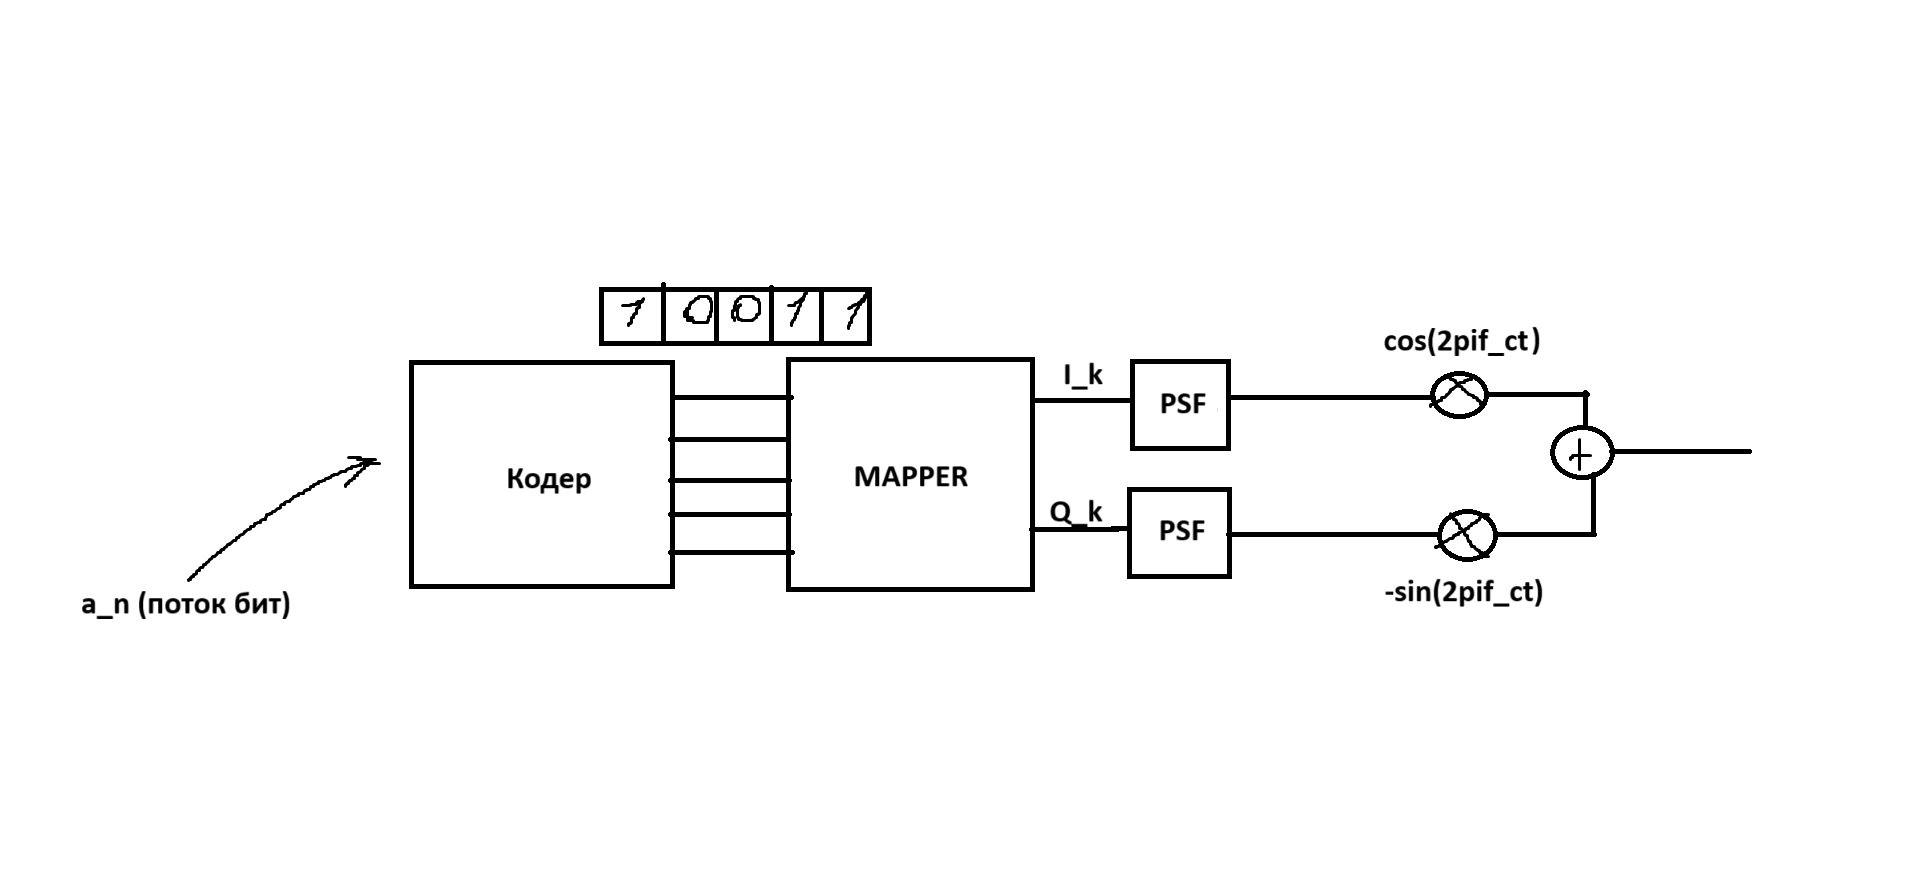
\includegraphics[width=1.0\textwidth]{tx_arch.png}
    \caption{Визуализация архитектуры передатчика}
\end{figure}

\section*{\textbf{Техническая реализация Upsampling}}

Техническую реализацию проще будет показать на примере. \\

Пусть на выходе маппера мы получили $I$ = [1, -1, 1], и хотим, чтобы каждый символ длился L = 4 семпла\\

Сформируем новую последовательность X(n), в которой между каждым $I_n$ добавим L-1 нулей.

\begin{figure}[H]
    \centering
    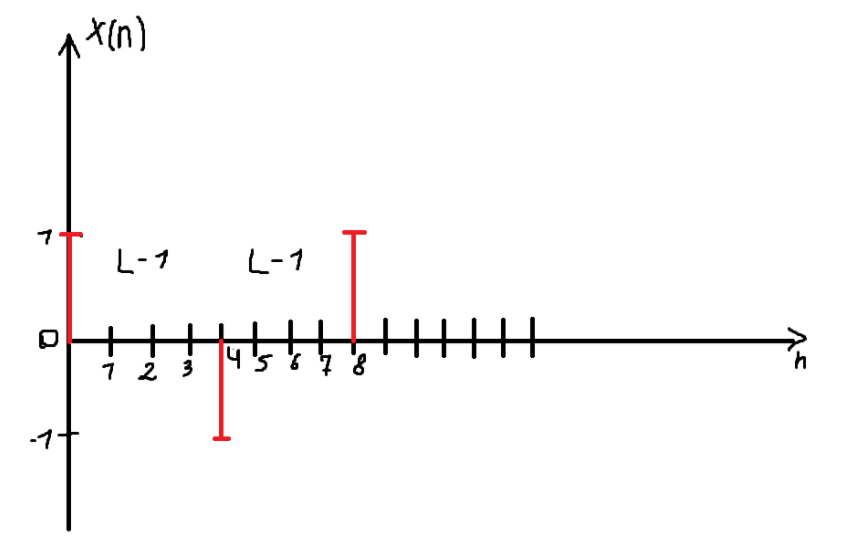
\includegraphics[width=1.0\textwidth]{Xn.png}
    \caption{Визуализация работы Upsampling}
\end{figure}

Получаем последовательность длинной 12 отсчетов (после последнего символа тоже идет 3 нуля).

\section*{\textbf{Формирующий фильтр}}

На данный момент мы только "растянули" символы, но не придали им никакой формы. Эти действия выполняет формирующий фильтр (на схеме g(n)). \\

В блоке g(n) происходят следующие расчеты: S(n) = $\sum_{m = 0}^{L-1}X(m)g(n-m)$, где X(n) - отсчеты, g(n) - импульсная характеристика фильтра.
Сама формула это дискретная свертка. \\

Импульсная характеристика фильтра имеет сложную форму, которая позволяет сделать сигнал любой формы. \\

Зададим форму импульсной характеристики. Для упрощения возьмем прямоугольную форму.

\begin{figure}[H]
    \centering
    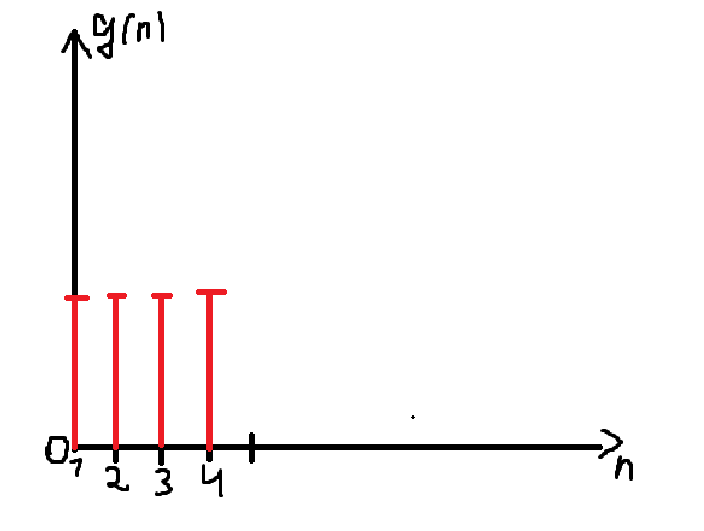
\includegraphics[width=1.0\textwidth]{gn.png}
    \caption{Пример импульсной характеристики}
\end{figure}

Для иллюстрации работы фильтра произведем вычисления по формуле выше:\\

S(0) = X(0)g(0) = 1*1 = 1\\

S(1) = X(0)g(1) + X(1)g(0) = 1*1 + 0*1 = 1 \\

S(2) = X(0)g(2) + X(1)g(1) + X(2)g(0) = 1*1 + 0*1 + 0*1 = 1 \\

S(3) = X(0)g(3) + X(1)g(2) + X(2)g(1) + X(3)g(0) = 1*1 + 0*1 + 0*1 + 0*1 = 1\\

S(4) = X(0)g(4) + X(1)g(3) + X(2)g(2) + X(3)g(1) + X(4)g(0) = 1*0 + 0*1 + 0*1 + 0*1 + (-1 * 1) = -1\\

S(4) = X(0)g(5) + X(1)g(4) + X(2)g(3) + X(3)g(2) + X(4)g(1) + X(5)g(0) = 1*0 + 0*0 + 0*1 + 0*1 + (-1 * 1) + 0 * 1 = -1\\

Визуализируем символы после выхода из фильтра:

\begin{figure}[H]
    \centering
    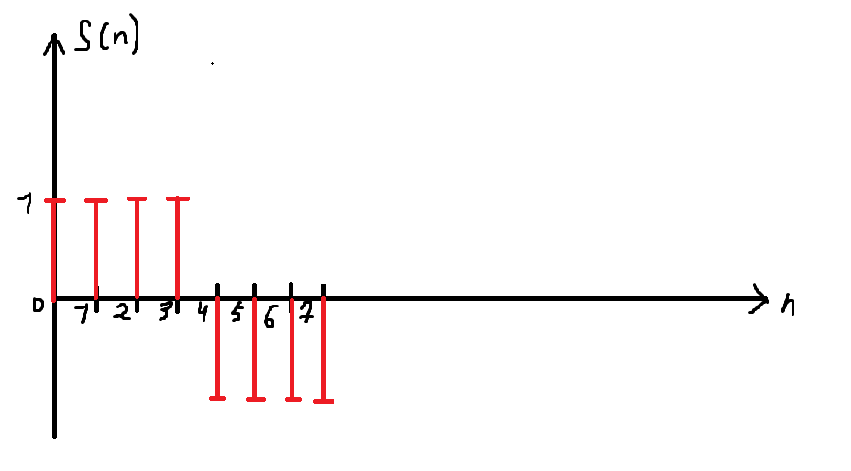
\includegraphics[width=1.0\textwidth]{sn.png}
    \caption{Пример символов после выхода из фильтра}
\end{figure}

Получили растянутые во времени I и Q с прямоугольной формой. Таким образом можно задать сигналу любую форму.

\endinput

                                     % Первая глава
\chapter{Практика}
\label{ch:chap2}

% \subsection*{\textbf{Здание 1: простой сигнал с 1 компонентой с нулевой начальной фазой}}

% Релизация задания в файле \textbf{task1.py} \\

% Результат: \\

% \begin{figure}[H]
%     \centering
%     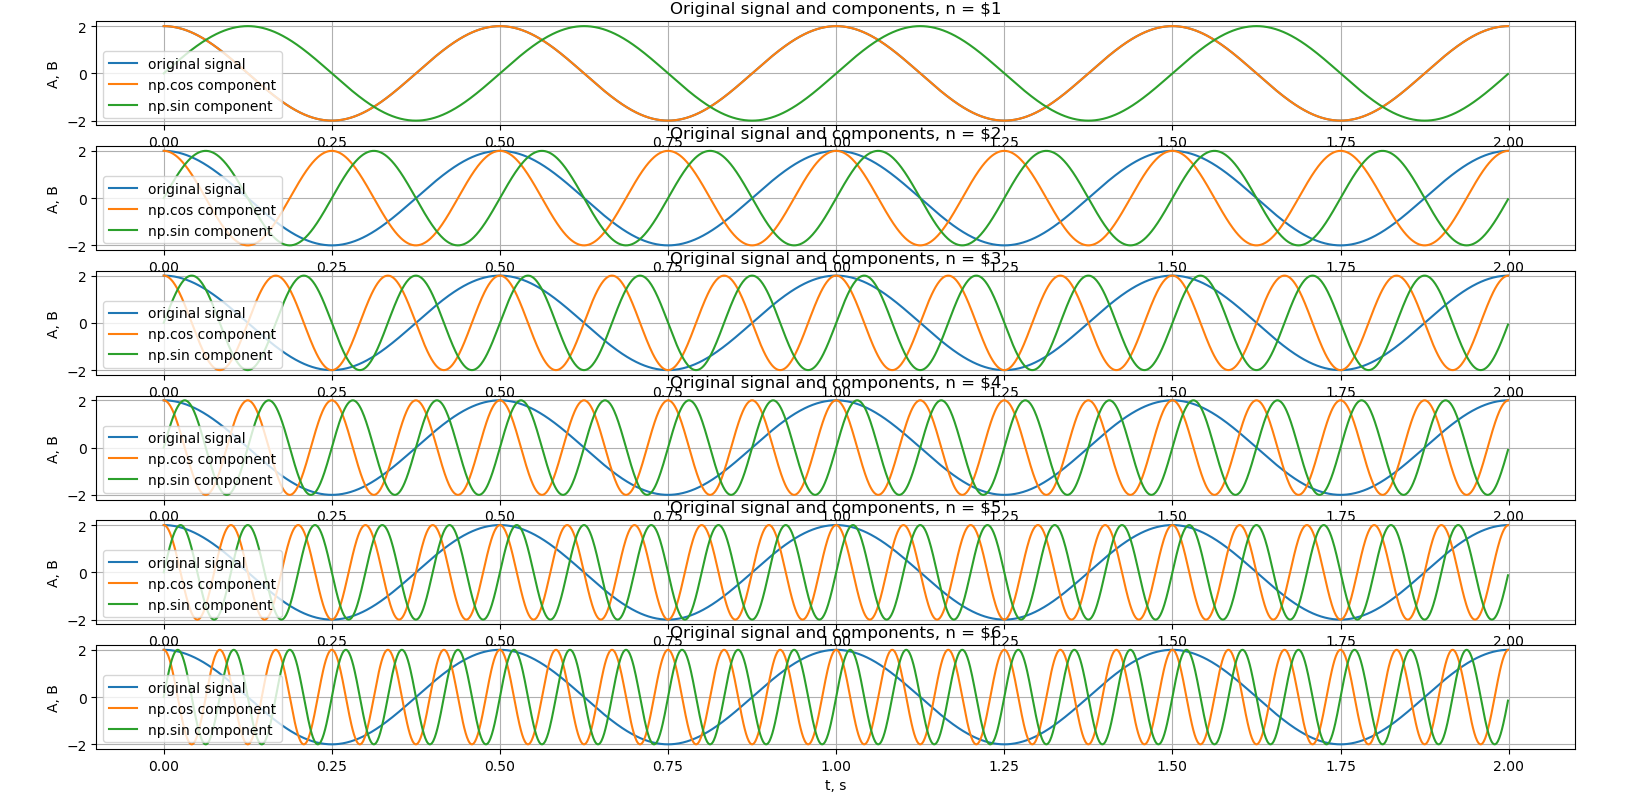
\includegraphics[width=1.0\textwidth]{task1_comp.png}
%     \caption{Графики оригинального сигнала и компонент}
% \end{figure}

% \begin{figure}[H]
%     \centering
%     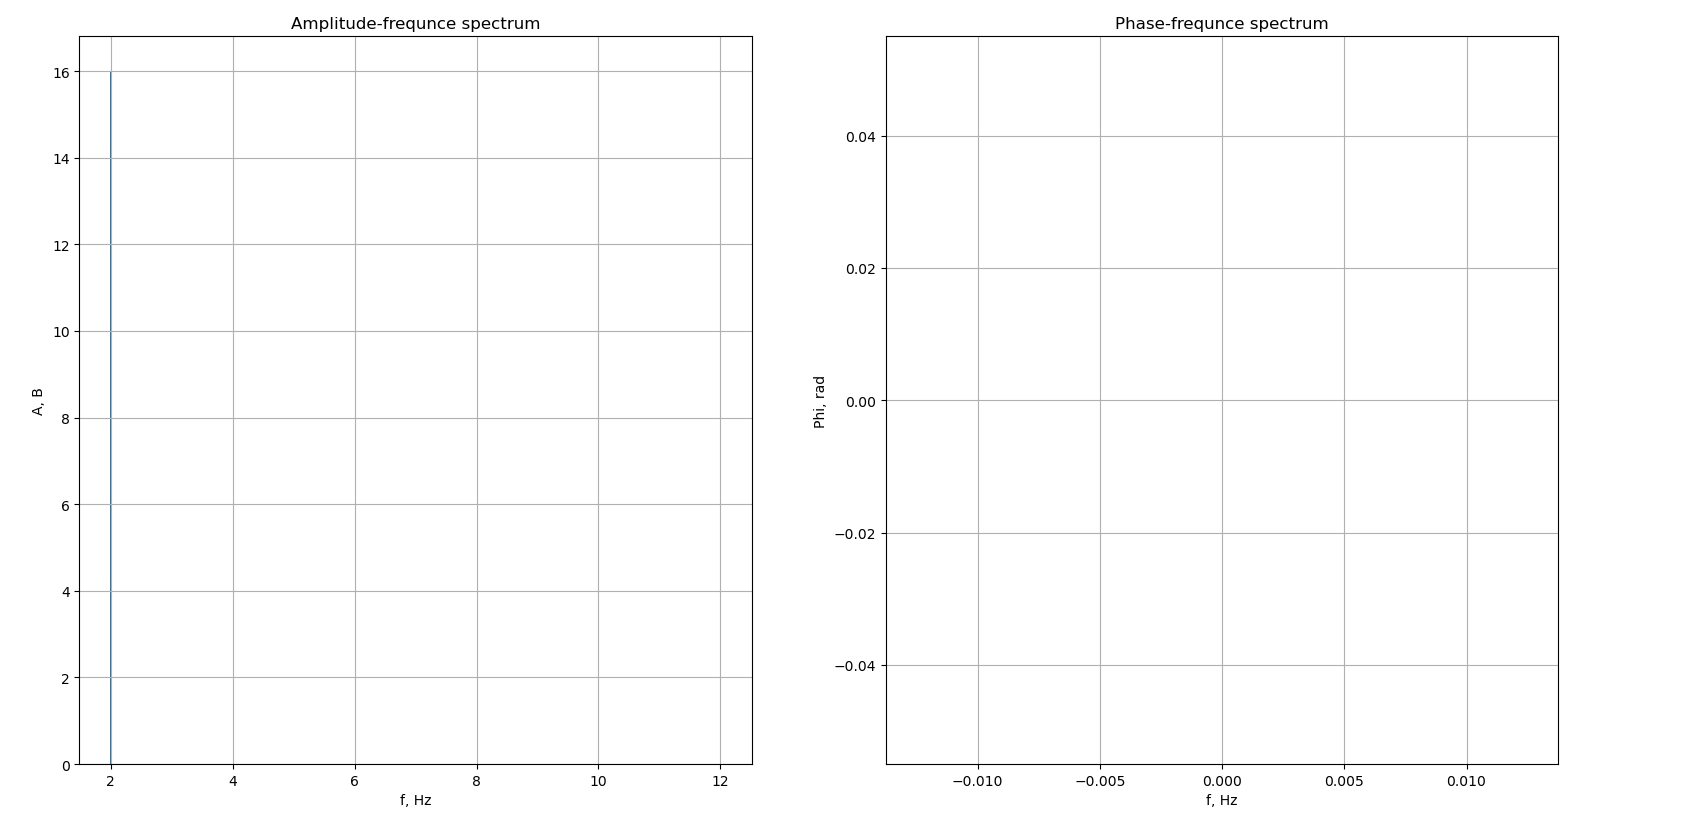
\includegraphics[width=1.0\textwidth]{task1_spec.png}
%     \caption{АЧХ и ФЧХ сигнала}
% \end{figure}

% По АЧХ можем наблюдать, что в сигнале есть 1 компонента с часоттой 2Гц, именно такой сигнал
% я изначально и задавал.

% \subsection*{\textbf{Здание 2: простой сигнал с 2 компонентами с нулевой начальной фазой}}

% Релизация задания в файле \textbf{task2.py} \\

% Результат: \\

% \begin{figure}[H]
%     \centering
%     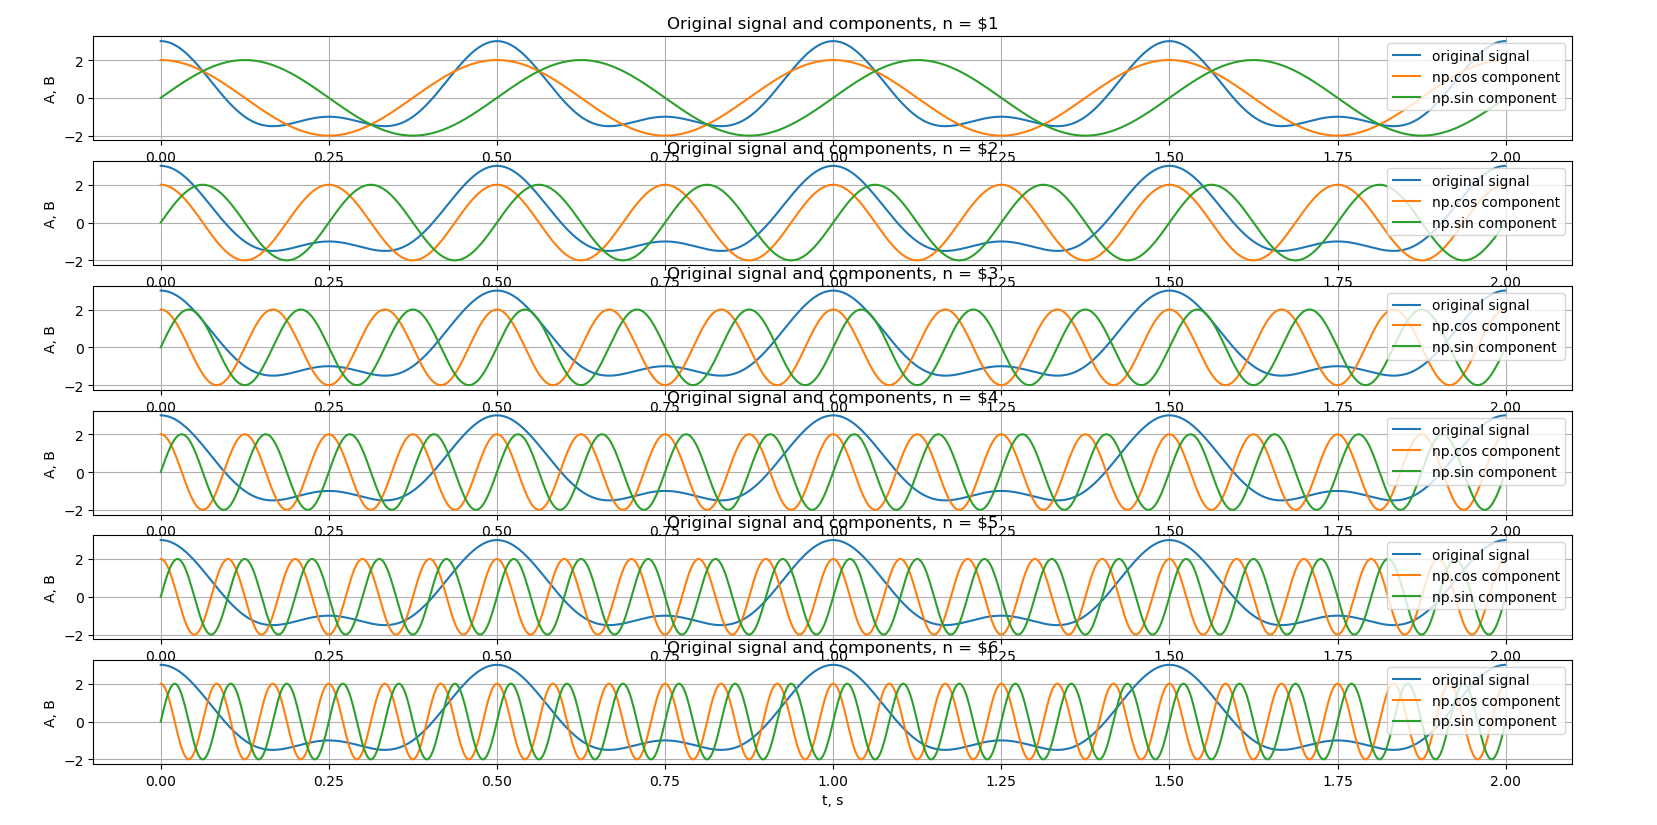
\includegraphics[width=1.0\textwidth]{task2_comp.png}
%     \caption{Графики оригинального сигнала и компонент}
% \end{figure}

% \begin{figure}[H]
%     \centering
%     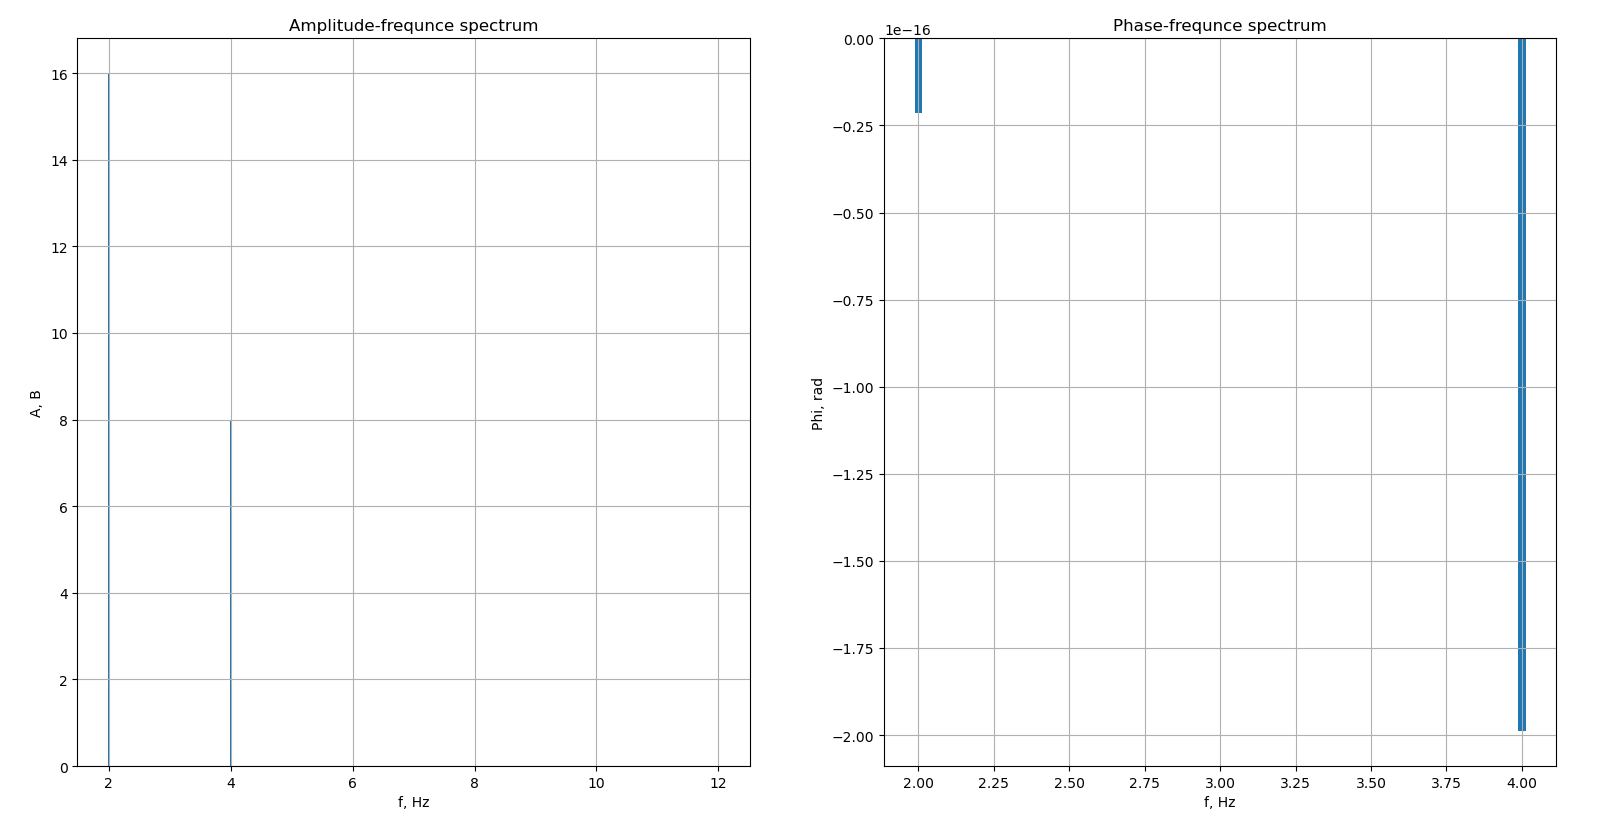
\includegraphics[width=1.0\textwidth]{task2_spec.png}
%     \caption{АЧХ и ФЧХ сигнала}
% \end{figure}

% По АЧХ можем наблюдать, что в сигнале есть 2 компоненты с часоттой 2 и 4 Гц, именно такой сигнал
% я изначально и задавал. На ФЧХ графике ложные фазы (это связано со свойствами acrtan).

% \subsection*{\textbf{Здание 3: простой сигнал с 2 компонентами с ненулевой начальной фазой}}

% Релизация задания в файле \textbf{task3.py} \\

% Результат: \\

% \begin{figure}[H]
%     \centering
%     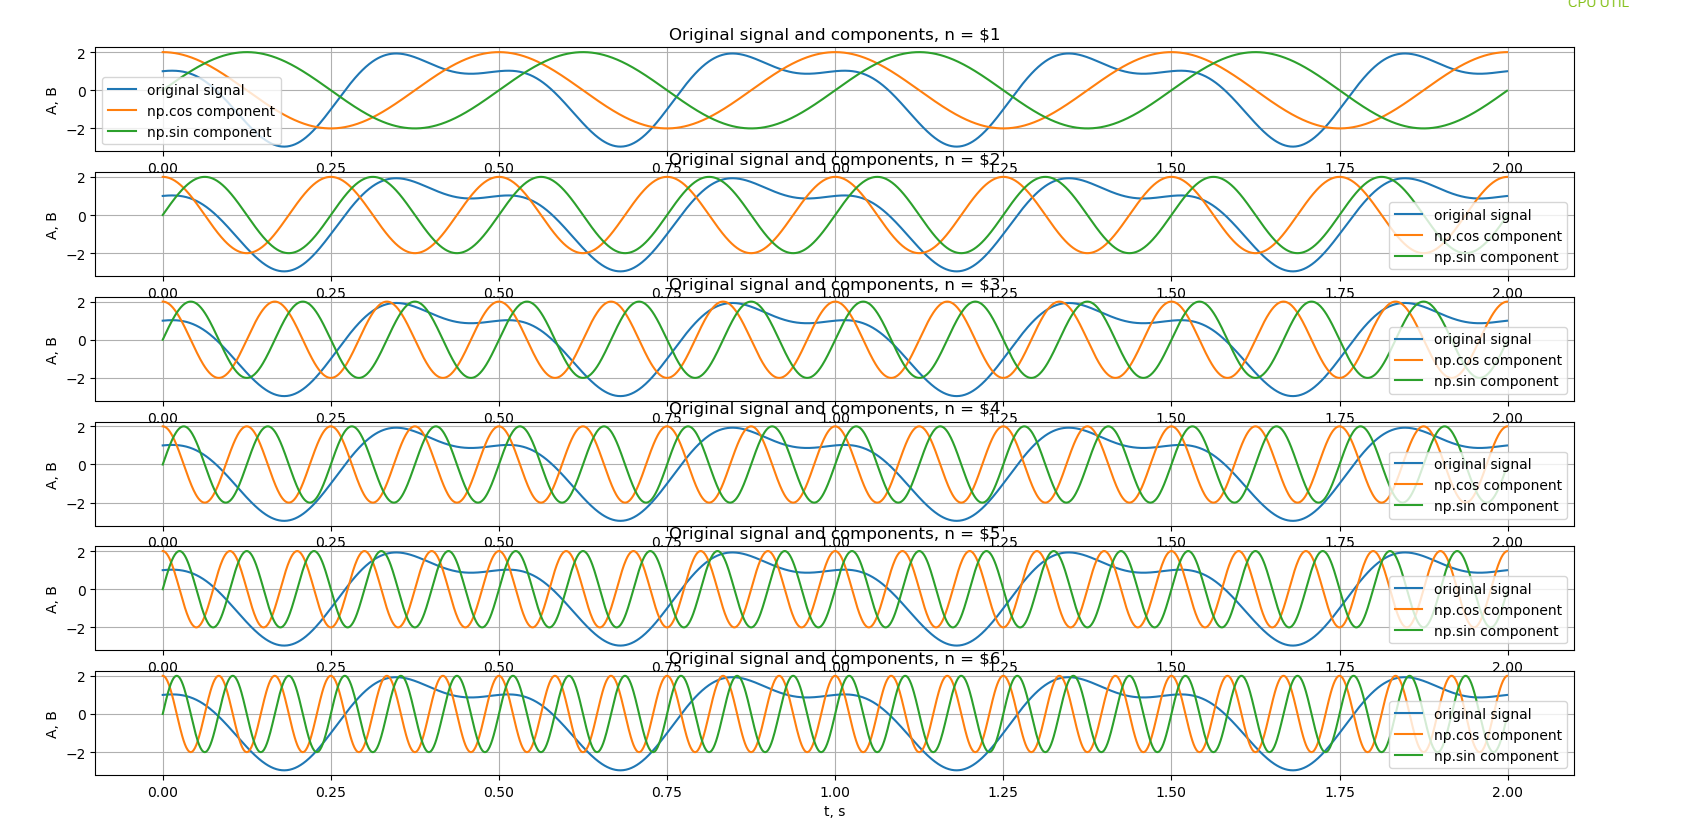
\includegraphics[width=1.0\textwidth]{task3_comp.png}
%     \caption{Графики оригинального сигнала и компонент}
% \end{figure}

% \begin{figure}[H]
%     \centering
%     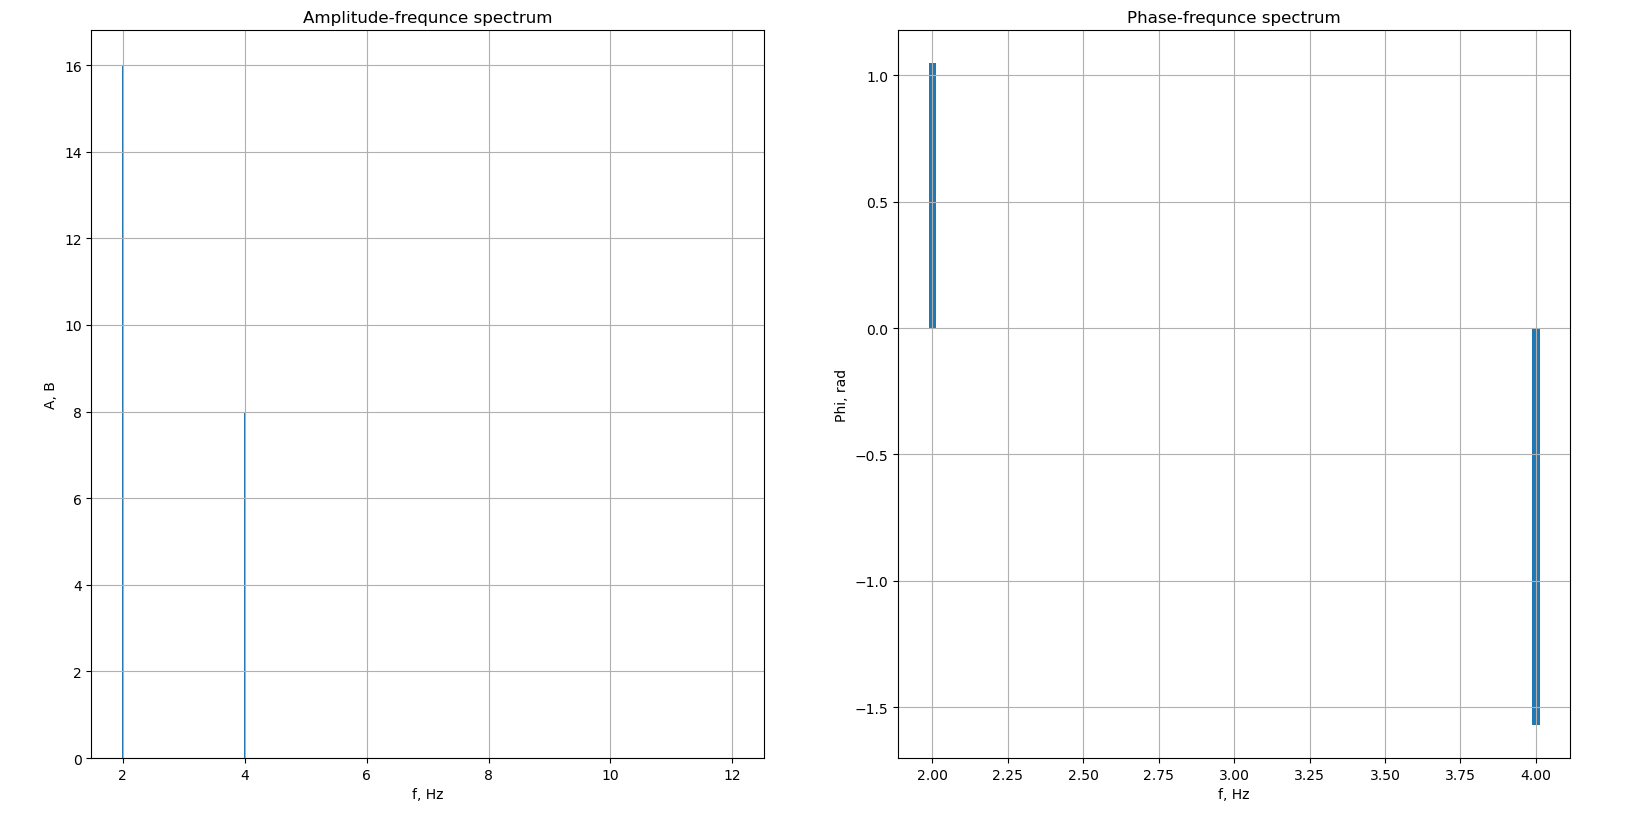
\includegraphics[width=1.0\textwidth]{task3_spec.png}
%     \caption{АЧХ и ФЧХ сигнала}
% \end{figure}

% По АЧХ можем наблюдать, что в сигнале есть 2 компоненты с часоттой 2 и 4 Гц, именно такой сигнал
% я изначально и задавал. На ФЧХ видим фазу $\pi/3$ для компоненты на 2Гц и $-\pi/3$ на 4 Гц, точно такой
% сигнал я и задавал.

% \subsection*{\textbf{Здание 4: прямоугольный сигнал}}

% Релизация задания в файле \textbf{task4.py} \\

% Результат: \\

% \begin{figure}[H]
%     \centering
%     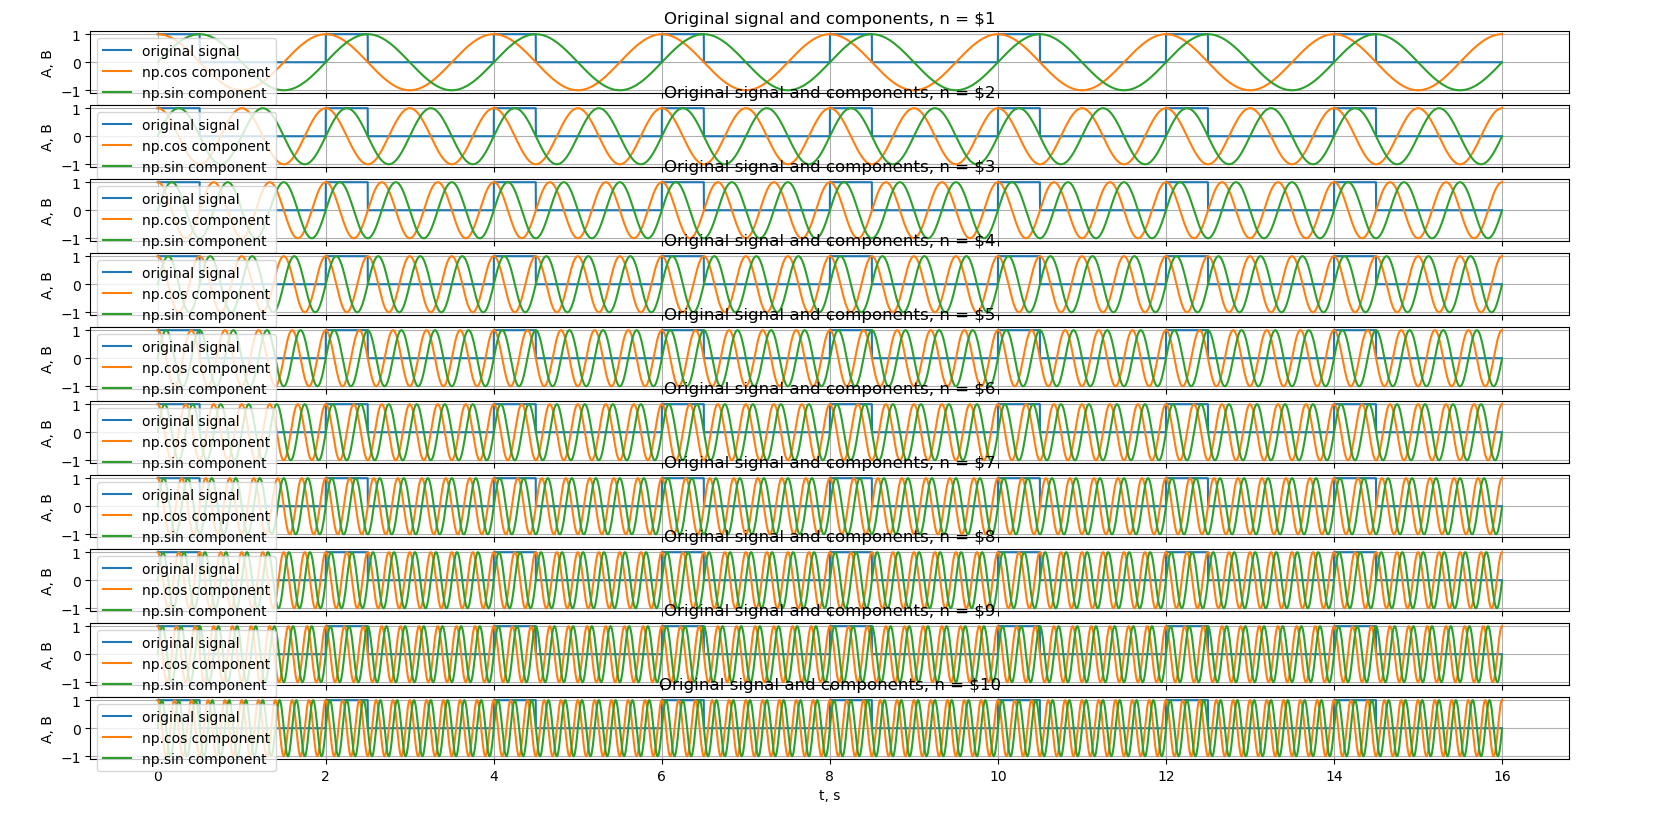
\includegraphics[width=1.0\textwidth]{task5_comp.png}
%     \caption{Графики оригинального сигнала и компонент}
% \end{figure}

% \begin{figure}[H]
%     \centering
%     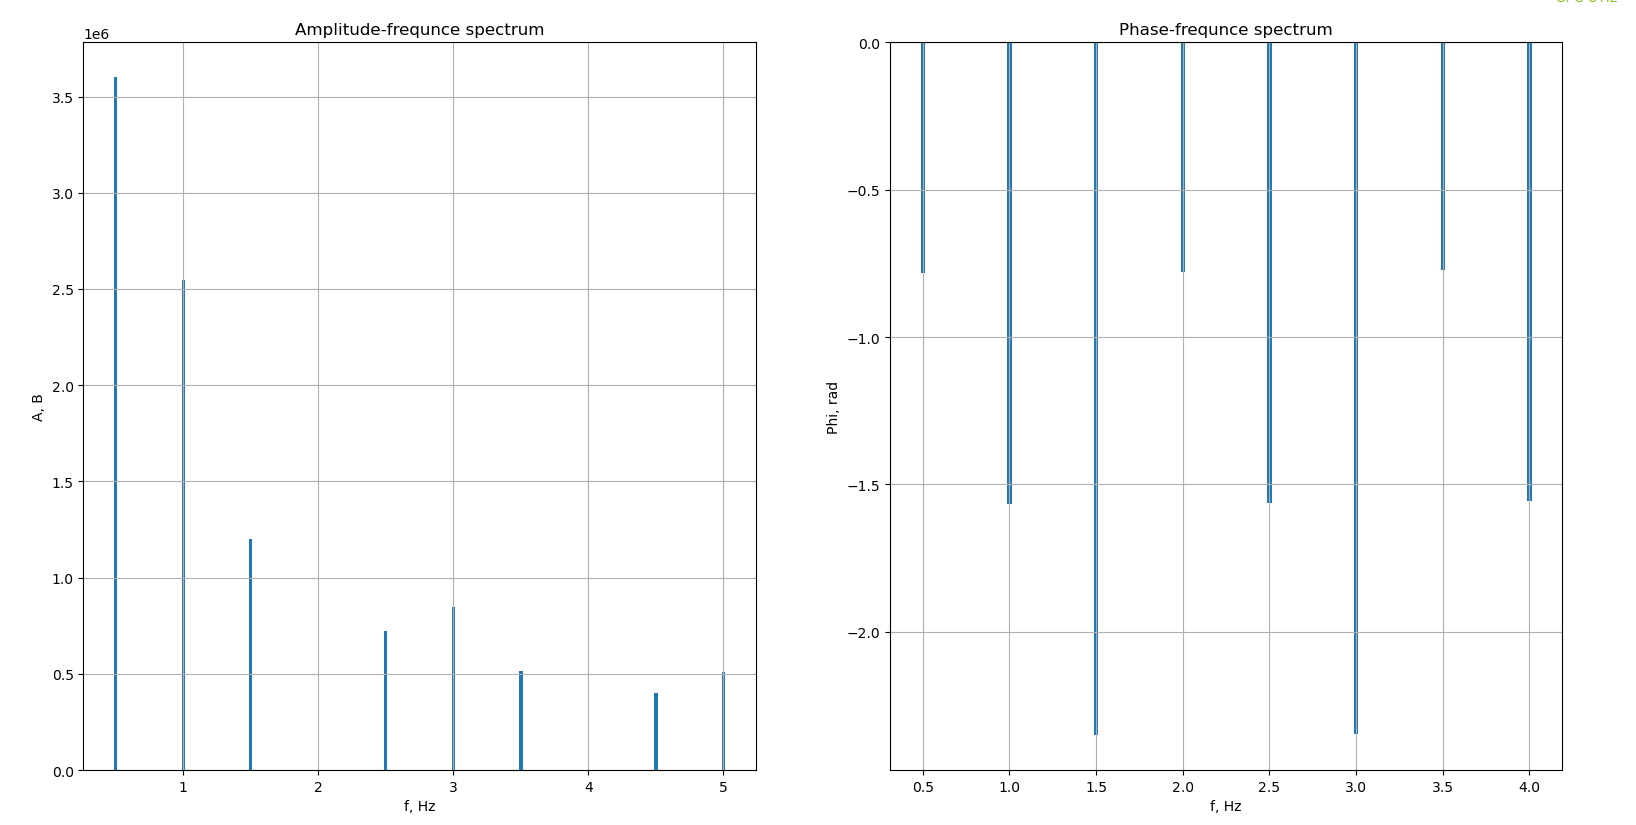
\includegraphics[width=1.0\textwidth]{task5_spectrum.png}
%     \caption{АЧХ и ФЧХ сигнала}
% \end{figure}

% По АЧХ можем наблюдать, что в сигнале есть 2 компоненты с часоттой 2 и 4 Гц, именно такой сигнал
% я изначально и задавал. На ФЧХ видим фазу $\pi/3$ для компоненты на 2Гц и $-\pi/3$ на 4 Гц, точно такой
% сигнал я и задавал. \\

% Теперь по полученным фазам и амплитудам попытаемся восстановить сигнал:

% \begin{figure}[H]
%     \centering
%     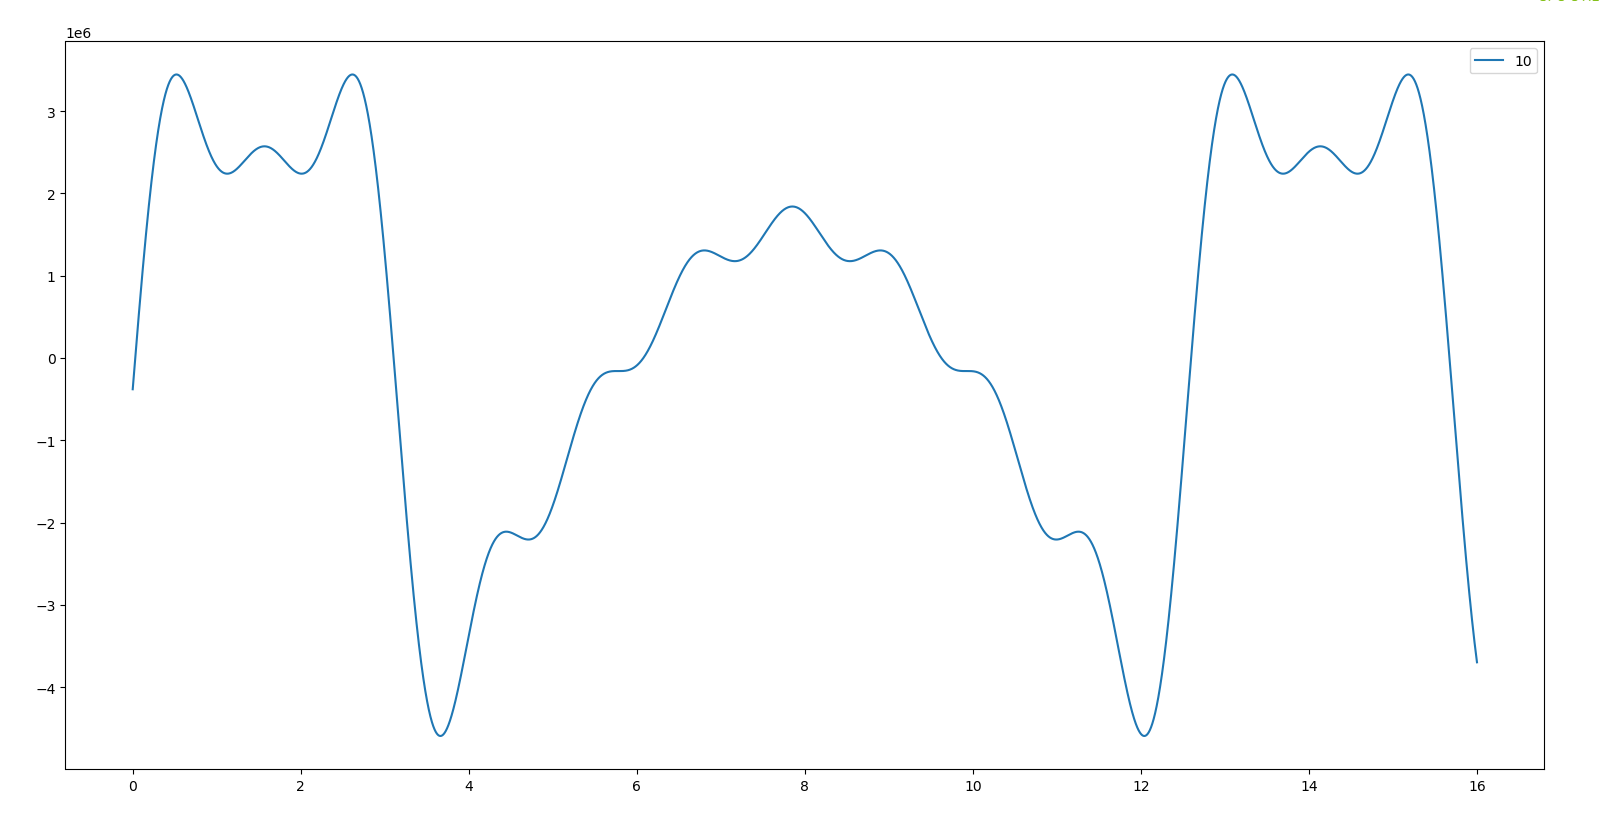
\includegraphics[width=1.0\textwidth]{ift.png}
%     \caption{Пример восстановленного сигнала}
% \end{figure}

% Сигнал не очень похож на прямоугольный, но можно заметить, что по бокам он начинает приобретать прямоугольную форму.

% \subsection*{\textbf{Здание 5: проверка ортогональности сигнала}}

% Релизация задания в файле \textbf{task5.py} \\

% Результат: \\

% \begin{figure}[H]
%     \centering
%     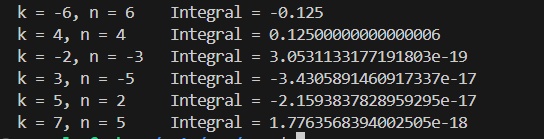
\includegraphics[width=1.0\textwidth]{task5_1.png}
%     \caption{Проверка ортогональности при интегрировании по периоду}
% \end{figure}

% k и n - коэффициенты при частотах sin сигналов, у которых проверяется ортогональнось. \\

% Заметим, что интеграл не равен нулю, когда n и k равны по модулю. Из этого можно сделать вывод о том, что 2 sin сигнала
% ортогональны, если их частоты по модулю не равны. \\

% Теперь сменим границы интегрирования. До этого интеграл был от 0 от Т, теперь будет от 0 до T+0.3:

% \begin{figure}[H]
%     \centering
%     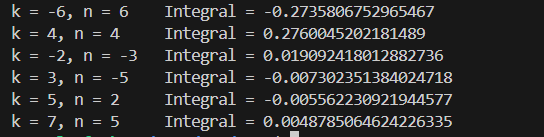
\includegraphics[width=1.0\textwidth]{task5_2.png}
%     \caption{Проверка ортогональности при интегрировании не по периоду}
% \end{figure}

% Можем заметить, что интегралы ненулевые. Из этого следует, что ортогональность соблюдается только при рассмотрении сигналов
% на периоде.

% \textbf{Примечание:} целых нулевых значений не получилось из-за ошибок округления и прочего. Числа с $e^{-n}$ - машинный 0.

% \subsection*{\textbf{Здание 6: разложение в комплексный ряд Фурье периодического прямоугольного сигнала}}

% Вычислим разложение в ряд Фурье для сигнала с разными параметрами:

% \begin{figure}[H]
%     \centering
%     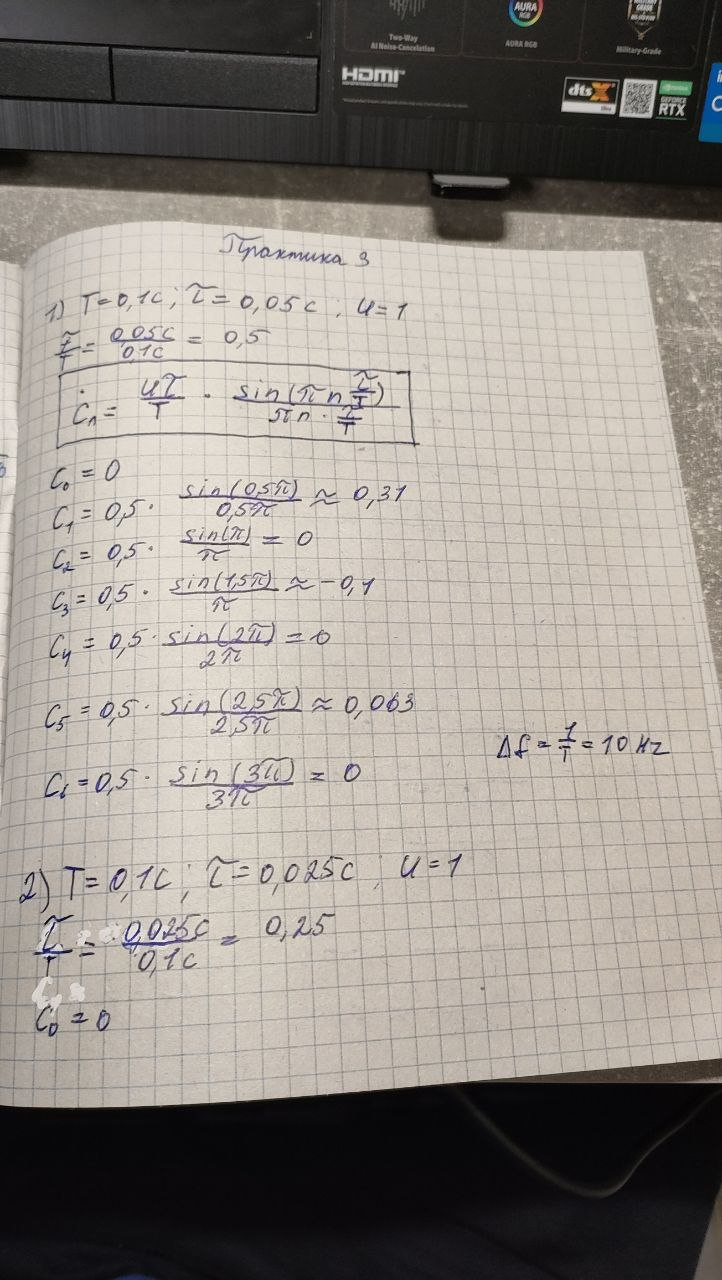
\includegraphics[width=1.0\textwidth]{comp1.png}
%     \caption{Разложение в ряд Фурье прямоугольного сигнала (расчеты)}
% \end{figure}

% \begin{figure}[H]
%     \centering
%     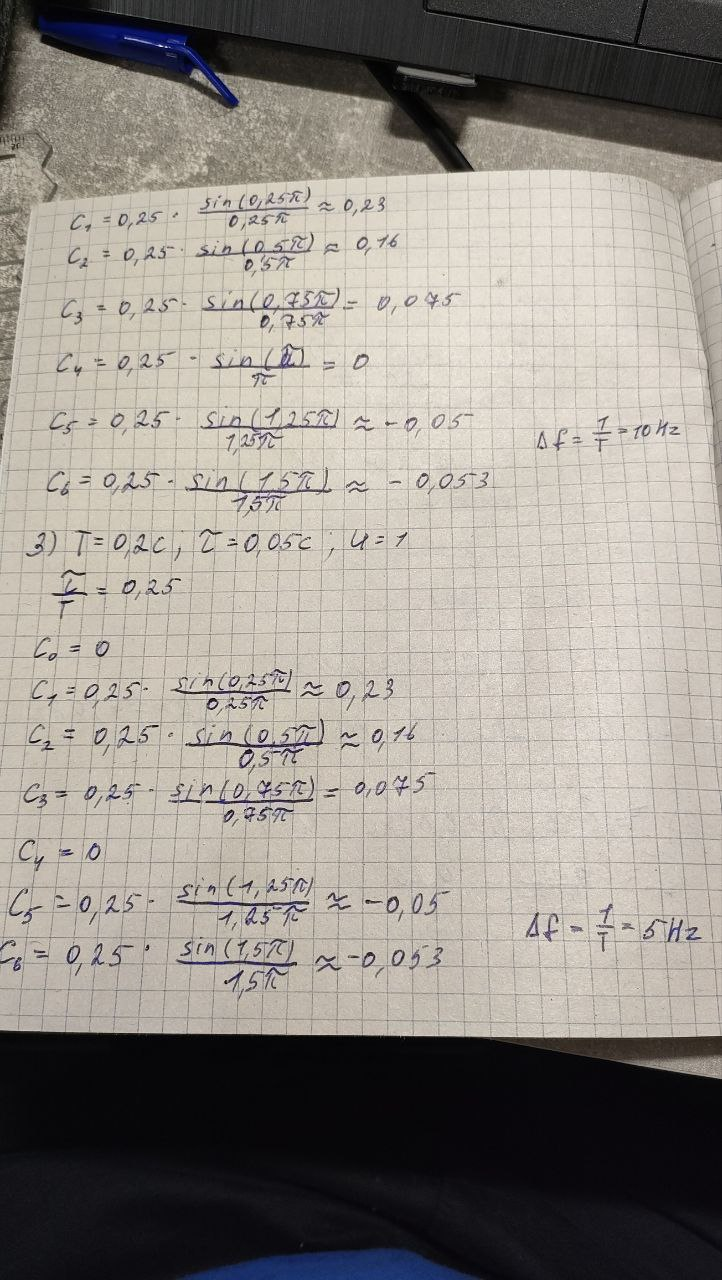
\includegraphics[width=1.0\textwidth]{comp2.png}
%     \caption{Разложение в ряд Фурье прямоугольного сигнала (расчеты)}
% \end{figure}

% Построим график АЧХ:

% \begin{figure}[H]
%     \centering
%     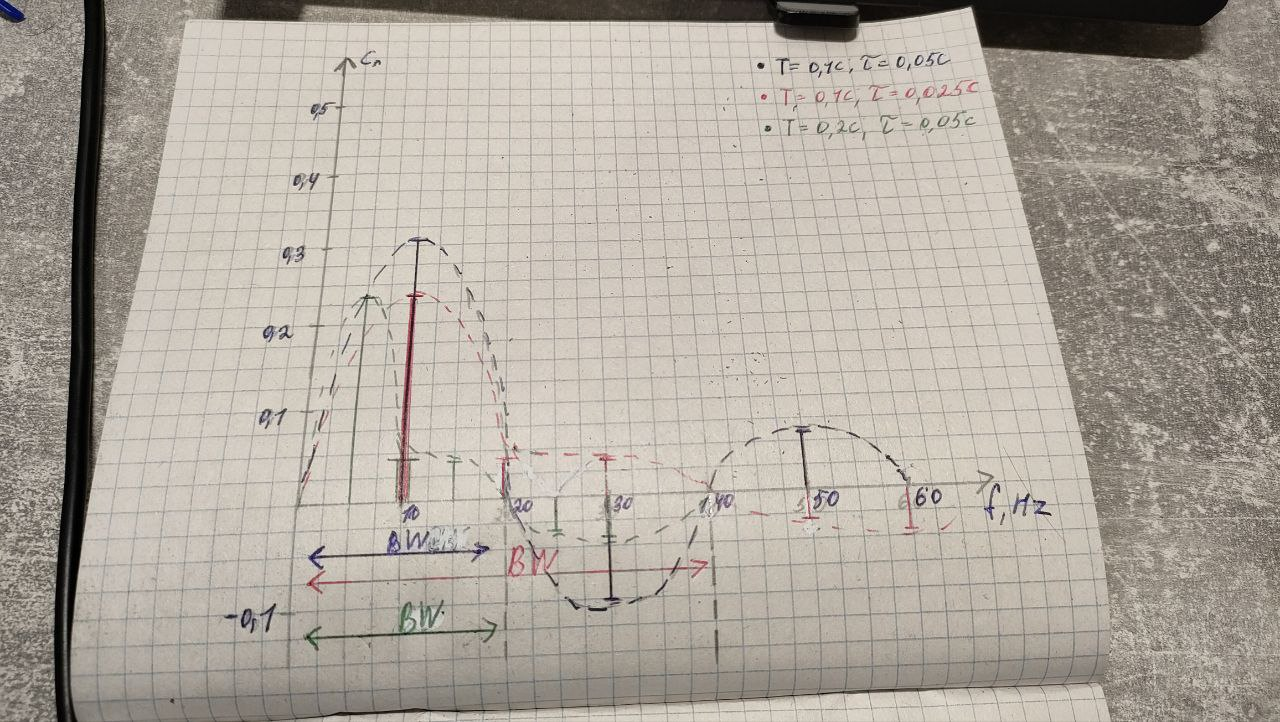
\includegraphics[width=1.0\textwidth]{plot.png}
%     \caption{График АЧХ}
% \end{figure}

% Можем заметить, что при уменьшении $\tau$ в 2 раза ширина спектра увеличилась вдвое, т.е ширина спектра обратно пропорциональна
% $\tau$. При этом в спектре сигнала стало больше гармоник, и у каждой амплитуда стала меньше (энергия перераспределилась). \\

% Еще можно заметить, что при увеличении периода T число гармоник не меняется, их амплитуды тоже остаются прежними, но сами 
% гармоники сдвинулись в область низких частот. Ширина спектра остается прежней.

\endinput                                     % Вторая глава                                 % Четвертая глава
\chapter{Вывод}
\label{ch:сhap5}

В ходе работы я изучил свойства преобразования Фурье и проверил их на практике.


\endinput  

\printbibliography[title=Список использованных источников] % Автособираемый список литературы

\end{document}